\documentclass[notitlepage]{report}
\usepackage[left=1in, right=1in, top=1in, bottom=1in]{geometry}

\usepackage{graphicx}
\usepackage{amsmath}

% Title Page Theme
\usepackage{titling}
\pretitle{\begin{center}\Huge\bfseries}
\posttitle{\par\end{center}\vskip 0.5em}
\preauthor{\begin{center}\Large\ttfamily}
\postauthor{\end{center}}
\predate{\par\large\centering}
\postdate{\par\vskip 1em}

\title{A Software Defined Modem Using Commodity Micro-Controllers}
\author{Joshua Jerred}
\date{\today}

\begin{document}
\maketitle

\begin{abstract}
  Modems, devices used to convert digital signals to and from analog signals are traditionally implemented using dedicated hardware, locking them to a specific modulation mode. With the rise of Software Defined Radio (SDR) and the increasing power of common micro-controllers (MCUs), generic hardware can be used to create a software defined modem. With the implementation of data modulation and demodulation in software, a single chip can be used for multiple communication modes, agnostic of hardware and a physical medium. Using the affordable STM32F4, along with it's analog-to-digital (ADC) converters, digital-to-analog (DAC) converters, direct-memory-access (DMA), and hardware timers, a multi-mode modem can be implemented.
\end{abstract}
  
\section{Introduction}

Commodity micro-controllers (MCUs), are capable of completing a wide variety of tasks thanks to their integrated hardware. This project aims to utilize the hardware built into a generic MCU to create a software defined modem. This modem will be capable of modulating and demodulating audio signals, agnostic of the physical medium and specific modulation mode. This will show that a commodity MCU  Although this project will focus on an older modulation mode, AFSK, the goal is to show that a modern MCU is powerful enough, given it's rich feature set, to fully implement a software defined modem without the need for any additional hardware.

\section{Background}

\subsection{Existing Work}

Software Defined Radio (SDR) is a term used to describe radio hardware that can be configured in software. This provides greater flexibility and allows for the use of a single piece of hardware for many purposes. The power of SDR was shown throughout the SpeakEasy, a project started in 1991 to help the United States Military address problems related to interoperability between branches\cite{speakeasy}. The project showed that a combination of hardware and software could be used to create a radio system that can be configured to operate on many different frequencies and modulation modes. Previously this had to be done with unique hardware for each mode.

When it comes to specifically using an MCU for this purpose, there are existing implementation. An article posted in ARRL QST in october of 1998 described using a PIC MCU to create AX.25 (describe ax.25) frames audio\cite{hansen_ax25}. These frames were then processed and made ready to be modulated into audio. The step of generating the audio was not implemented in this article, but the author suggested using external hardware or a MCU capable of generating audio. This article does show that a MCU can at least be used to generate the data that is to be modulated into audio.

There is a implementation of AFSK audio generation using an Arduino (ATmega 2560)\cite{arduino_afsk}. In this implementation, the AFSK generation was done in software with a interrupt being triggered for each sample of the audio stream. Demodulation was not implemented in this project.

\subsection{AFSK}

\subsection{ADC/DAC/DMA}

\subsection{Existing Work} % Change the name of this section, doesn't seem right.


\section{Hardware}
Newer devices, such as the STM32, have powerful ARM cores matched up with other hardware inside of small single chip MCU packages. With peripherals like ADCs and DACs, along side DMA, audio can be cleanly generated in real time. This can be used to generate modulated data streams, with one common piece of hardware.

Although using a Digital Signal Processor (DSP) would be useful... more here

The idea of this project is that a generic microcontroller (MCU) is capable of acting as a software defined modem. Given this, the hardware will be kept simple. A single MCU will be used to act as the software modem. The modem will be connected to an external host/client, this client will control the modem. The modem has a single audio output and audio input, this can connected to various types of physical mediums to transfer the data that is modulated in the audio from one modem to another.


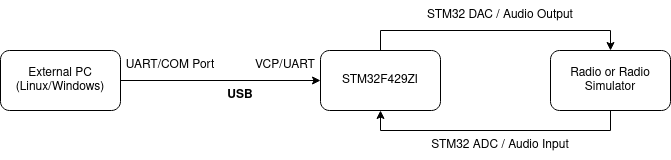
\includegraphics[width=4in]{images/hardware_outline}

\begin{center}
\subsection{MCU Requirements/Considerations}
\end{center}

When looking for the appropriate MCU for this project there were a few requirements and considerations that needed to be taken into account.

\begin{itemize}
  \item[ADC] A single ADC (Analog-to-Digital Converter) is required to sample the input audio. It needs suitable resolution and speed to capture the modulated audio stream.
  \item[DAC] A single DAC (Digital-to-Analog Converter) is required to output modulated audio from the microcontroller.
  \item[DMA] DMA (Direct Memory Access) is required to transfer data to/from the ADC/DAC automatically without CPU intervention. Although this may not be strictly required, it will free up a considerable amount of CPU time.
  \item[Hardware Timers] Accurate hardware timers are required for properly timing the audio waveform generation, and the modulation.
  \item[USB/UART] A USB/UART connection is required to connect an external MCU to a host device so that the host device can send/receive data to/from the modem.
  \item[Cost] There are many devices that are capable of completing the task, but the cost of the device is a major consideration. The device should be as cheap and as generic as possible to allow for easy replication of this project on other hardware.
\end{itemize}

The STM32F4 series of MCUs are a good fit for this project as they are fast, contain all of the required components, and they are cheap. These are fairly generic MCUs that are available for \$.

\section{Software Implementation}
\subsection{AFSK Introduction}
AFSK, or Audio-Frequency-Shift-Keying, is a method of encoding bits into a modulated audio signal. This is done by modulating a carrier wave between two frequencies, where each distinct frequency represents a symbol. For this Implementation there will be two symbols, 1 and 0, at 1200 Hz and 2200 Hz respectively. The rate at which symbols change can be variable, but 1200 baud was chosen for this project. This is the same method used by the Bell 202 modem.

EXAMPLE IMAGE OF AFSK

\subsection{Waveform Generation}
Any method of audio modulation requires that a waveform be generated. This waveform is then modified to represent unique symbols. Therefore, a MCU must be able to generate a simple sine wave. With AFSK being the primary modulation mode for this project, a 1200 Hz wave is generated.

The goal was to have the MCU generate a constant sine wave without a large impact to CPU usage. Using the DAC, alongside DMA, and a hardware timer. The DAC will output a constant voltage given a constant 12-bit value. Utilizing an array of sine wave values, the DMA will transfer the values to the DAC at a constant rate set by a hardware timer. A single cycle of the sine wave is represented by 128 12-bit values. Given this information, and a hardware clock, the timer can be configured to trigger at a rate that will generate a sine wave at a given rate. For example, the timer configuration for a 1200hz sine wave is as follows:

\[
  F_{trigger} = \frac{C_{APB1}}{(PSC+1)*(ARR+1)}
\]
where:
\begin{itemize}
  \item[$C_{APB1}$] is the clock frequency of the APB1 bus (90 MHz)
  \item[$PSC$] is the prescaler value
  \item[$ARR$] is the auto-reload value
  \item[$F_{trigger}$] is the frequency of the trigger (1200 Hz)
\end{itemize}

\[
  F_{output} = \frac{F_{trigger}}{N_{samples}}
\]

IMAGE OF OUTPUT

This method provides a constant sine wave output with no CPU intervention past configuring the DAC on startup, and configuring/starting the timer. After this, the CPU is free to do other tasks.

\subsection{Modulation}

Modulation is the process of converting raw data, bits, into a modulated audio signal. This is done by taking a raw data stream, and generating the proper audio samples. The modem will look at each bit in order, and change the audio output frequency depending on the value of the bit. Provided the implementation of the waveform generation, the act of changing frequencies only requires changing the hard clock configuration, specifically the ARR and PSC values in software. For modulation, another hardware timer was used. This is configured to trigger a software interrupt at the baud rate of the modem. This interrupt will then read the next bit in the data stream, and set the frequency of the output waveform accordingly. As the baud rate is 1200, this interrupt will be triggered at 1200 Hz.

By utilizing the hardware built into the MCU, modulation can be done with minimal CPU intervention allowing the single-core MCU to perform other tasks, like external communication, while modulating audio.

IMAGE OF MODULATION - create a timeline graphic that shows the hardware interrupts

\subsection{Demodulation}

\subsection{External Communication}

\section{Testing}

\section{Conclusion}

\bibliographystyle{plain}
\bibliography{refs}

\end{document}